\documentclass[12pt]{article}
\usepackage{bigpage}
\usepackage{blockpar}
\usepackage{amsmath}
\usepackage{hyperref}
\usepackage{graphicx}
\usepackage{xfrac}

\title{The Usual Derivation of Neural Net Backpropagation}
\author{Bart Massey}
\date{2012/11/13}

\newcommand{\yhat}{{\hat y}}
\renewcommand{\d}{\partial}
\renewcommand{\dh}{{\partial h}}
\newcommand{\Half}{{\frac 1 2}}
\newcommand{\half}{{\sfrac 1 2}}
\newcommand{\ehh}{{e^{\half - h}}}

\begin{document}
\maketitle
This treatment mostly follows
\url{http://www.doc.ic.ac.uk/~nd/surprise_96/journal/vol4/cs11/report.html}.
I used the open source computer algebra package Maxima
(\url{http://maxima.sourceforge.net}) to do
and check some of the math.

Consider a neuron that looks like this:
\begin{quotation}
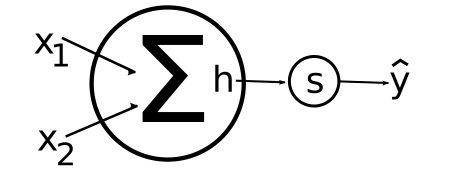
\includegraphics[height=0.6in]{neuron.pdf}
\end{quotation}

We start with the axiomatic definitions. We will assume that
all inputs to a neuron are in the interval $[-1\ldots 1]$
and that the output will be in the same range. Our squashing
function is the symmetric version of the sigmoid.  Our first
goal is to try to pick weights to minimize the mean squared
error $E$ between the desired output $y$ and the actual
output $\yhat$.

\begin{align}
x_i, \yhat &\in [-1..1] \\
h &= \sum_i{w_i x_i} \\
s &= \frac{e^h - 1}{e^h + 1} \\
\yhat &= s \circ h \\
E(y, \yhat) &= \Half (\yhat - y)^2
\end{align}

We now compute a couple of derivatives that will be
interesting in error analysis. Note how the derivative of
the {\bf htan} squashing function $s$ is a simple
function of {\bf htan}.  This is convenient in the
implementation, since it means that we can use a single
routine for both training and classification.

\begin{align}
E_y &= \frac{\d E}{\d \yhat} \\
    &= \yhat - y
\end{align}
\begin{align}
E_\yhat &= \frac{\d \yhat}{\dh} \\
    &= \frac{\d s(h)}{\dh} \\
    &= \frac{\frac \d \dh {(e^h - 1)} \cdot (e^h + 1) -
       (e^h - 1) \cdot \frac \d \dh {(e^h + 1)}}{(e^h + 1)^2} \\
    &= \frac{e^h (e^h + 1) - (e^h - 1) e^h}{(e^h + 1)^2} \\
    &= \frac{e^h (e^h + 1 - e^h + 1)}{(e^h + 1)^2} \\
    &= \frac{2 e^h}{(e^h + 1)^2} \\
    &= \Half \frac{4 e^h}{(e^h + 1)^2} \\
    &= \Half \frac{\left ({e^h}^2 + 2e^h + 1 \right ) -
                   \left ( {e^h}^2 - 2e^h + 1 \right )}{(e^h + 1)^2} \\
    &= \Half \frac{({e^h} + 1)^2 -
                   ({e^h}^2 - 1)^2}{(e^h + 1)^2} \\
    &= \Half \left ( 1 - \left ( \frac{e^h - 1}{e^h +1} \right )^2\right ) \\
    &= \Half \left ( 1 - s^2(h) \right ) \\
    &= \Half \left ( 1 - \yhat^2  \right )
\end{align}

This is a convenient conclusion, since it allows us to
compute the derivative $E_\yhat$ using just $\yhat$ itself.

Next, we compute the error due to weight $w_i$ and
due to input $x_i$. We use the chain rule on the previously
calculated derivatives.

\begin{align}
E_{w_i} &= \frac{\d E}{\d w_i} \\
    &= \frac{\d E}{\d \yhat} \cdot
       \frac{\d \yhat}{\dh} \cdot
       \frac{\d h}{\d {w_i}} \\
    &= E_y \cdot E_\yhat \cdot \frac{\dh}{\d {w_i}} \\
    &= (\yhat - y) \cdot \Half (1 - \yhat^2) \cdot
       x_i  \label{eqn-Ewi}
\end{align}
\begin{align}
E_{x_i} &= \frac{\d E}{\d x_i} \\
    &= \frac{\d E}{\d h} \frac{\d h}{\d x_i} \\
    &= (\yhat - y) \cdot \Half (1 - \yhat^2) \cdot w_i \label{eqn-Exi}
\end{align}

At this point, we can use $E_{w_i}$ to adjust the weights,
and then use $E_{x_i}$ to find error terms for the prior;
that is, for the outputs from the previous network layer.

Another legitimate choice would have been to have chosen to
have $x_i$ and $\yhat$ in the range $[0..1]$. This is the
more common choice in the literature.

The math is the same, except that we now use a slightly
different squashing function. Specifically, we want the
squashing function to have a range $y = [0..1]$, half the
previous range with $\half$ offset; we also want the
squashing function to have its center at $x = \half$ instead
of at $x = 0$

\begin{align}
s(h) &= \Half \frac {e^{h - \half} - 1}  {e^{h - \half} + 1} + \Half \\
     &= \Half \left ( \frac {e^{h - \half} - 1} {e^{h - \half} + 1} + 1 \right ) \\
     &= \Half \frac {e^{h - \half} - 1 + e^{h - \half} + 1} {e^{h - \half} + 1} \\
     &= \frac {e^{h - \half}} {e^{h - \half} + 1} \\
     &= \frac 1 {1 + \ehh}
\end{align}

This new function has a slightly different derivative.

\begin{align}
E_\yhat &= \frac{\d \yhat}{\dh} \\
    &= \frac{\d s(h)}{\dh} \\
    &= \frac \d \dh {\left [{(1 + \ehh)}^{-1} \right ]} \\
    &= -{(1 + \ehh)}^{-2} \cdot \frac \d \dh {(1 + \ehh)} \\
    &= \frac{\ehh}{(1 + \ehh)^2} \\
    &= \frac{\ehh + 1 - 1}{(\ehh + 1)^2} \\
    &= \frac 1 {\ehh + 1} - \frac 1 {(\ehh + 1)^2} \\
    &= \frac 1 {\ehh + 1} \left ( 1 - \frac 1 {\ehh + 1} \right ) \\
    &= s(h) (1 - s(h)) \\
    &= \yhat (1 - \yhat)
\end{align}

The adjustment to equations \ref{eqn-Ewi} and \ref{eqn-Exi}
is just rework, and is left to the reader.
\end{document}
